\documentclass[oribibl]{llncs}

%\usepackage{pslatex}

\usepackage{times}
\usepackage{amsmath}
\usepackage{amsfonts}
\usepackage{amssymb}
\usepackage{mathpartir} % ./
\usepackage{color}
\usepackage{xspace} 
\usepackage[pdftex]{graphicx}
%\usepackage[small]{caption}
\usepackage{fancybox}
\usepackage{url}
\usepackage{multirow}
\usepackage{comment}
\usepackage{listing}
\usepackage{colortbl}
\usepackage{subfigure}

%\usepackage{times}
\usepackage{framed}
\usepackage{lineno}

%!TEX root =  main.tex

\newcommand{\cvc}{\textsc{cvc}{\small 4}\xspace}
\newcommand{\cvciii}{\textsc{cvc}{\small 3}\xspace}
\newcommand{\ziii}{\textsc{z}{\small 3}\xspace}
\newcommand{\teq}{\approx}
\newcommand{\cc}[1]{#1^*}
\newcommand{\M}{\mathcal{M}}
\def\AIF{\qtab\keyword{if}\ }
\def\THEN{\ \keyword{then}\ }
\def\AELSE{\untab\qtab\keyword{else}\ }
\def\FI{\untab}
\def\RETURN{\keyword{return}\ }
\def\ENDPROC{\untab}
%\newtheorem{remark}{Remark}


\newcommand{\define}[1]{\textsl{#1}}
\newcommand{\defas}{\stackrel{\mathrm{def}}{=}}

\newcommand{\rem}[1]{\textcolor{magenta}{[#1]}}
\newcommand{\remvk}[1]{\textcolor{red}{[#1]}}
\newcommand{\ct}[1]{\rem{#1 --ct}}
\newcommand{\ajr}[1]{\rem{#1 --ajr}}
\newcommand{\vk}[1]{\remvk{#1 --vk}}

\newcommand{\terms}{\mathbf{T}}
\newcommand{\sorts}{\mathbf{S}}
\newcommand{\vals}{\mathbf{V}}
\newcommand{\vars}{\mathbf{X}}
%\newcommand{\sorts}{\mathsf{sort}}
\newcommand{\funcs}{\mathsf{func}}

\newcommand{\I}{\mathcal{I}}
\newcommand{\J}{\mathcal{J}}
\newcommand{\Iu}{I}
\newcommand{\mods}{\mathbf{I}}
\newcommand{\lan}{\mathbf{L}}
\newcommand{\qlan}[1]{\mathcal{Q}( #1 )}
\newcommand{\props}{\mathbf{P}}

\newcommand{\modsof}[2]{{\llbracket {#1} \rrbracket}_{#2}}

\newcommand{\ent}[1][]{\models_{#1}}
\newcommand{\tent}{\ent[T]}

\newcommand{\ssorts}[1]{#1^\mathrm{s}}
\newcommand{\sfuns}[1]{#1^\mathrm{f}}

\newcommand{\con}[1]{\mathsf{#1}}
\newcommand{\Bool}{\con{Bool}}
\newcommand{\Int}{\con{Int}}
\newcommand{\Real}{\con{Real}}
\newcommand{\ite}{\con{ite}}
\newcommand{\ev}{\con{ev}}
\newcommand{\size}{\con{size}}

\newcommand{\TD}{T_\mathrm{D}}

\newcommand{\ltrue}{\top}
\newcommand{\lfalse}{\bot}

\newcommand{\euf}{\ensuremath{\mathrm{EUF}}\xspace}
\newcommand{\tra}{\ensuremath{\mathrm{RA}}\xspace}
\newcommand{\tia}{\ensuremath{\mathrm{IA}}\xspace}
\newcommand{\lra}{\ensuremath{\mathrm{LRA}}\xspace}
\newcommand{\lia}{\ensuremath{\mathrm{LIA}}\xspace}
\newcommand{\lira}{\ensuremath{\mathrm{LIRA}}\xspace}
\newcommand{\uflia}{\ensuremath{\mathrm{UFLIA}}\xspace}
\newcommand{\larel}{\bowtie}

\newcommand{\nmf}[1]{#1\negthinspace\downarrow}
\newcommand{\interp}[1]{[ \negthinspace [ #1 ] \negthinspace ]}

\newtheorem{thm}{Theorem}
\newtheorem{cor}{Corollary}
\newtheorem{lem}{Lemma}
\newtheorem{defn}{Definition}
%\newtheorem{claim}{Claim}

\newcommand{\opdivd}{\small\mathsf{div}}
\newcommand{\opdivl}{\small\mathsf{div}^{-}}
\newcommand{\opdivu}{\small\mathsf{div}^{+}}
\newcommand{\opmod}{\xspace \mathsf{mod} \xspace}
\newcommand{\oplcm}{\xspace \mathsf{lcm} \xspace}
\newcommand{\opdivides}{\xspace \mid \xspace}
\newcommand{\opliapol}{b}
\newcommand{\optoint}{\small\mathsf{to\_int}}

\newcommand{\funcsolve}{\small\mathsf{solve}}
\newcommand{\funcsmtsolve}{\small\mathsf{DPLL_{\forall T}}}
\newcommand{\funcqi}{\small\mathsf{check}_\forall}

\newcommand{\Set}[1]{\left\{#1\right\}}
\newcommand{\parens}[1]{\left(#1\right)}
\newcommand{\tuple}[1]{\left\langle#1\right\rangle}

\newcommand{\bigor}{\bigvee}
\newcommand{\bigand}{\bigand}

\newcommand{\divides}{\mid}
\newcommand{\notdivides}{\nmid}
\newcommand{\fvars}{FV}

\newcommand{\normalize}[1]{{#1}\!\!\downarrow}
\newcommand{\intnormalize}[1]{{#1}\!\!\downarrow_{\Int}}
\newcommand{\unnormalize}[2]{{#1}\!\!\updownarrow^{#2}}
\newcommand{\approxg}[2]{{#1}\!\!\mid_{#2}}

\newcommand{\transform}{\ \leadsto \ }

\newcommand{\purify}[1]{\lfloor #1 \rfloor}
\newcommand{\purifyrec}[1]{\purify{#1}^\ast}
\newcommand{\purifyg}[3]{\purify{#1}_{(#2,#3)}}
\newcommand{\unpurify}[1]{\lceil #1 \rceil}
\newcommand{\quants}[1]{\mathcal{Q}(#1)}
\newcommand{\guardspos}[1]{\mathcal{A}(#1)}
\newcommand{\guardsneg}[1]{\mathcal{B}(#1)}
\newcommand{\activequants}[2]{\mathrm{Q}(#1,#2)}
\newcommand{\lits}{\#\mathsf{lits}}
\newcommand{\opmax}{\mathsf{max}}
\newcommand{\opmin}{\mathsf{min}}

\renewcommand{\shadowsize}{1pt}

\begin{document}

\title{Conflicts, Models and Heuristics for Quantifier Instantiation in SMT}

\author {Andrew Reynolds\inst{1}}

\institute{
Department of Computer Science, The University of Iowa, USA
}
\maketitle

\pagestyle{plain}
%\pagestyle{empty}

\begin{abstract}
Satisifiability Modulo Theories (SMT) solvers have
emerged as prominent tools in formal methods applications.
While originally targetted towards quantifier-free inputs,
SMT solvers have gained significant use for quantified formulas in automated
theorem proving and software verification.
The most common technique for handling quantified formulas in modern SMT solvers
in quantifier instantiation.
This paper gives an overview of recent advances in quantifier instantiation in SMT.
In addition to the well-known technique known as E-matching,
we discuss the use of conflicts and models for 
accelerating the search for (un)satisfiably.
We further mention new instantiation-based techniques
that are specialized to background theories such as linear real and integer arithmetic.
\end{abstract}

\section{Introduction}

[SMT solvers now handle quantifiers]
Satisifiability Modulo Theories (SMT) solvers 


The use of quantified formulas is highly important in a number of applications.
Among these, in automated theorem proving applications~\cite{},
quantified formulas
In software verification~\cite{},

In synthesis~\cite{},

In planning~\cite{},


Unfortunately, reasoning about quantified formulas is very challenging in theory, and
in only limited cases does the satisfiability problem remain decidable.


In spite of the theoretical challenges, quantified formulas
can be handled well in practice by modern automated theorem provers and SMT solvers.



A growing number of modern tools exist for reasoning about first-order quantified formulas.
A number of automated theorem provers
such as Vampire~\cite{DBLP:conf/cav/KovacsV13}, E~\cite{schulz2002brainiac}, and SPASS~\cite{weidenbach2009spass})
were developed to target quantified formulas in single-sorted first-order logic.
More recently, these solvers have been extended with dedicated support for background theories~\cite{}.
For the most part, theorem provers from this community are superposition-based,
although some are instantiation-based such as the Inst-Gen calculus used by iProver~\cite{ganzinger2003new}.
A recent approach known as AVATAR~\cite{DBLP:conf/cade/RegerSV15} leverages support in SAT and SMT solvers for quantifier-free formulas
in combination with a superposition-based theorem prover.

In contrast to most of these automated theorem provers, 
SMT solvers such as CVC~\cite{stump2002cvc}, Yices~\cite{dutertre2006yices}, and Z3~\cite{Z3}, 
were originally developed to target quantifier-free formulas in background theories,
but have more recently been extended with support for universally quantified formulas.
The approaches here are mostly instantiation-based based~\cite{Detlefs03simplify:a,MouraBjoerner07,GeBarrettTinelli07},
although some approaches are based on superposition~\cite{de2008engineering}.

This paper will focus primarily on recent techniques for quantifier instantiation in SMT solvers.
In Section~\ref{sec:quant}, we outline an abstract procedure used by most SMT solvers with support for quantified formulas.
We then focus on three general-purpose instantiation strategies for handling quantified formulas in SMT:
\begin{itemize}
\item Section~\ref{sec:ematching} will discuss \emph{heuristic} techniques for quantifier instantiation based on pattern-matching that
are widely-used by current solvers,
\item Section~\ref{sec:cbqi} will discuss how finding \emph{conflicts} can improve the ability of solvers to answer ``unsat",
\item Section~\ref{sec:mbqi} will examine how constructing candidate \emph{models} can enable the solvers to answer ``sat".
\end{itemize} 
Section~\ref{sec:cegqi} introduces further techniques for quantifier instantiation in SMT that 
are specialized to theories.
Finally, we conclude in Section~\ref{sec:conclusion} with a summary and mention possible future work.

\section{Support for Quantified Formulas in an SMT Solver}
\label{sec:quant}

Most modern SMT solvers are based on the DPLL($T$) solving architecture,
where a set of decision procedures for $T$ are modularly combined with a SAT solver for propositional satisfiability~\cite{nieuwenhuis2006solving}.
Given a set of $T$-formulas $\Gamma$ as input to a DPLL($T$)-based SMT solver, its underlying SAT solver
abstracts each $T$-literal in $\Gamma$ as unique Boolean variable.
The SAT solver clausifies $\Gamma$ and returns that 
either $\Gamma$ is propositionally unsatisfiable (in which case it is also $T$-unsatisfiable),
or returns a set of literals $M$ that propositionally entail it.
We write $M \models_p \Gamma$ to denote this case, and refer to $M$ as a satisfying assignment for $\Gamma$.
It then uses a decision procedure for $T$ to
check the $T$-satisfiability of $M$, that is, whether there exists of model of $M$ that is consistent according to theory $T$.
If $M$ is $T$-satisfiable, then we may conclude that $\Gamma$ is $T$-satisfiable.
Otherwise, it returns a subset $C$ of $M$ that is $T$-unsatisfiable and adds the clause $\neg C$ to $\Gamma$,
which is often referred to as a conflict clause.

%In DPLL($T$), each theory literal and closed universally quantified formula is abstracted as a unique Boolean variable.
%The underlying SAT solver 

DPLL($T$)-based SMT solvers have been extended in the past decade with approaches for univeral and existential quantification~\cite{Detlefs03simplify:a,MouraBjoerner07,GeBarrettTinelli07}.
For consistency, in this paper we assume all existential quantification is rewritten to universal quantification by the rewrite:
\[
\exists \vec x\, P( \vec x ) \transform \neg \forall \vec x\, \neg P( \vec x )
\]
In a DPLL($T$)-based approach for quantified formulas, 
each closed (universally) quantified formula is abstracted as a Boolean variable by the SAT solver as well.

\begin{example}
Consider the set of $\uflia$-formulas:

\end{example}

\begin{figure}[t]
\begin{framed}
\begin{internallinenumbers}
$\funcsmtsolve( \Gamma )$:
\begin{enumerate}
\item[\ ] If $\Gamma$ is propositionally unsatisfiable,
\begin{enumerate}
\item[\ ] return ``unsat".
\end{enumerate}
\item[\ ] Otherwise, let $M = E \uplus Q$ be a set of literals such that $M \models_p \Gamma$.
\item[\ ] If $E$ is $T$-unsatisfiable,
\begin{enumerate}
\item[\ ] return $\funcsmtsolve( \Gamma \cup \neg C )$ for some $T$-unsatisfiable $C \subseteq E$.
\end{enumerate}
\item[\ ] Otherwise, let $( r, L ) = \funcqi( E, Q )$.
\item[\ ] If $r$ is ``unknown",
\begin{enumerate}
\item[\ ] return $\funcsmtsolve( \Gamma \cup L )$.
\end{enumerate}
\item[\ ] Otherwise, return ``sat".
\end{enumerate}
$\funcqi( E, Q )$:
\begin{enumerate}
\item[\ ] Do one of the following:
\begin{enumerate}
\item[\ ] Return $( \text{``unknown"}, L )$ for some set $L$ of $T$-lemmas.
\item[\ ] Return $( \text{``sat"}, \emptyset )$, if $E \cup Q$ is $T$-satisfiable.
\end{enumerate}
\end{enumerate}
\end{internallinenumbers}
\end{framed}
\vspace{-2ex}
\caption{An abstract procedure for $T$-inputs $\Gamma_0$ with quantified formulas in an SMT solver.
In Line 5, $E$ is quantifier-free, and the atoms of each literal in $Q$ are universally quantified formulas.
\label{fig:smtq}}
\end{figure}

Figure~\ref{fig:smtq} gives an abstract procedure $\funcsmtsolve$
for establishing the $T$-satisfiability of a set of $T$-formulas $\Gamma$ possibly containing universal quantification.
Lines 2 through 6 correspond to a DPLL($T$)-based approach for quantifier-free inputs.
In Line 5, we partition $M$ into two parts $E$ and $Q$,
where $E$ is quantifier-free and the atoms of literals in $Q$ are universally quantified formulas.
If the quantifier-free portion is $T$-satisfiable,
we proceed to Line 7, which invokes the procedure $\funcqi$ on $E$ and $Q$.
Abstractly, this procedure either may determine that $E \cup Q$ is $T$-satisfiable and return the pair $( \text{``sat"}, \emptyset )$,
or otherwise will return ( ``unknown", $L$ ), where $L$ is a set of formulas that are valid in theory $T$,
after which the procedure $\funcsmtsolve$ either terminates with ``sat" or adds $L$ to $\Gamma$ and repeats.

Designing support for quantified formulas in DPLL($T$)-based SMT solvers 
primarily depends on how the function $\funcqi$ is implemented.
We will examine such an implementation in this paper, in particular addressing the questions:
\begin{itemize}
\item How can we establish that $E \cup Q$ is $T$-satisfiable (when $Q$ is non-empty)?
\item What lemmas $L$ should we return?
\end{itemize}

It is important to note that some SMT approaches to quantified formulas
reason about quantified formulas \emph{eagerly} during the DPLL($T$) search~\cite{MouraBjoerner07}.
In terms of Figure~\ref{fig:smtq}, these approaches invoke $\funcqi$
when $M$ is incomplete and does not necessarily propositionally entail all formulas in $\Gamma$.
The advantage of doing so is that lemmas returned by $\funcqi$ may help prune the search,
while the disadvantage is that calling $\funcqi$ may be expensive.
%For simplicity, we assume a lazy approach for handling quantified formulas.

\subsection{Skolemization and Instantiation}
Common implementations of $\funcqi( E, Q )$ in SMT solvers return sets $L$ consisting of $T$-lemmas of the following two forms:
\begin{enumerate}
\item $\neg \forall \vec x\, P( \vec x ) \Rightarrow \neg P( \vec k )$, where $\vec k$ is a set of fresh \emph{Skolem} variables, and
\item $\forall \vec x\, P( \vec x ) \Rightarrow P( \vec t )$, where $\vec t$ is a tuple of ground terms.
\end{enumerate}
Lemmas of the first type, which we refer to as \emph{Skolemization lemmas},
 witness the negation of universally quantified formulas for a fresh set of variables $\vec{k}$,
are returned for each quantified formula whose negation occurs in $Q$.
Notice that such lemmas need only be added once per quantified formula.
Lemmas of the second type, which we refer to as \emph{instantiation lemmas},
infer an instance of a universally quantified formula for some tuple of ground terms $\vec{ t }$.
In contrast, multiple lemmas of this form may be added per quantified formula.
The performance of the solver is highly dependent on a having a good strategy for selecting instantiation lemmas.
We examine various strategies for selecting instantiation lemmas in Sections~\ref{sec:ematching}-~\ref{sec:cegqi}.

\section{E-matching}
\label{sec:ematching}

The most widely used technique for quantifier instantiation in SMT a heuristic technique known as \emph{E-matching}.
It was originally introduced in the Ph.D. thesis of Greg Nelson~\cite{Nelson:1980:TPV:909447}.
Recently, variants of the approach have been implemented in a number of solvers~\cite{Detlefs03simplify:a,DBLP:conf/cav/BarrettT07,Z3,DBLP:conf/cade/BoutonODF09,CVC4-CAV-11,DBLP:conf/lpar/Rummer12}.
The support for E-matching in these solvers is critical to the success of high-level tools for 
software verfication~\cite{DBLP:conf/icse/Leino04,DBLP:conf/itp/ChapmanS14} and automated theorem proving~\cite{blanchette2013extending,bobot2011why3}.
E-matching chooses instances for quantified formulas $\forall \vec x\, \varphi$
based on \emph{pattern terms} whose free variables are $\vec x$.
We will write $p[ \vec x ]$ to denote a term whose free variables are $\vec x$.
%Formally, 
%we say that a ground term $g$ matches $p$ modulo $E$ under substitution $\{ \vec x \mapsto \vec t \}$ if $E \models_T g = p \{ \vec x \mapsto \vec t \}$.
In detail, 
E-matching does the following for each $\forall \vec x\, \varphi[ \vec x ]$ in $Q$:
\begin{enumerate}
\item Choose a set of patterns $p_1[ \vec x ], \ldots, p_m[ \vec x ]$.
\item For each $j = 1, \ldots, m$,
\begin{enumerate}
\item Compute a set of pairs $(\vec t_{1},g_{1}), \ldots, (\vec t_{n}, g_{n})$ 
where for each $i = 1, \ldots, n$, we have that $g_i$ is a ground term from $E$ such that $E \models_T g_{i} = p_j[ \vec t_{i} ]$.
\item Return the lemmas $\{ \forall x\, \varphi[\vec x] \Rightarrow \varphi[\vec t_{1}], \ldots, \forall x\, \varphi[\vec x] \Rightarrow \varphi[\vec t_{n}] \}$.
\end{enumerate}
\end{enumerate}

In other words, we first select some set of pattern terms, which are often some of the subterms of $\varphi$.
For each of these patterns $p_j[ \vec x ]$, we compute a set of pairs of the form $( \vec t_i, g_i )$ where 
$g_i$ is equivalent to $p_j[ \vec t_i ]$ under the assumption that $E$ holds.
We then return instantiation lemmas corresponding to each of these pairs. 
In the context of Figure~\ref{fig:smtq}, these lemmas are included in the return value of $\funcqi$ (set $L$).
Notice in this description, we write $E \models_T g_{i} = p_j[ \vec t_{i} ]$ to denote that $E$ entails
$g_{i} = p_j[ \vec t_{i} ]$ modulo theory $T$.  In typical E-matching implementations, $T$ is limited to the theory of uninterpreted functions and equality.
%We demonstrate this technique in the following examples.

\begin{example}
\label{ex:em2}
Let $E$ be the set $\{ P(a), \neg P(b), R(c), \neg R(a), S(d) \}$ where $a,b,c,d$ are free constants and $P,R,S$ are unary predicates.
Let $\psi$ be $\forall x\, P( x ) \vee R( x )$.
Say we choose the pattern terms $P( x )$ and $R( x )$ for $\psi$.
In Step 2, we compute pairs $( a, P( a ) )$ and $( b, P( b ) )$ for $P( x )$ and
$( a, R( a ) )$ and $( c, R( c ) )$ for $R( x )$,
and E-matching returns $\{
\psi \Rightarrow P( a ) \vee R( a ), \psi \Rightarrow P( b ) \vee R( b ), \psi \Rightarrow P( c ) \vee R( c )
\}$.
\qed
\end{example}

\begin{example}
\label{ex:em2}
E-matching also takes into account matching modulo equality.
For example, let $E$ be the set $\{ P( a, c ), f( b ) = a \}$,
let $\psi$ be $\forall xy\, P( f( x ), y ) \Rightarrow g( x ) = y$,
and let $P( f( x ), y )$ be a pattern for it.
We may consider the pair $( ( b, c ), P( a, c ) )$, which is such that $E \models_\euf P( a, c ) = P( f( b ), c )$ since $f( b ) = a \in E$,
where $\models_\euf$ denotes entailment the theory of equality and uninterpreted functions.
E-matching in this example returns $\{ \psi \Rightarrow ( P( f( b ), c ) \Rightarrow g( b ) = c \}$.
\qed
\end{example}

Recall in function $\funcqi$, we are interested in the (un)satisfiability of $E \cup Q$.
As mentioned, E-matching selects instantiation lemmas based on pattern matching.
It is typically very effective for establishing unsatisfiability.
The intuition for its effectiveness is the following. 
Let $\psi$ be a formula in $Q$ of the form $\forall \vec x\, \varphi[ p[ \vec x ], \vec x ]$, 
that is, $p[ \vec x ]$ is a subterm of $\psi$,
Assume $p[ \vec x ]$ is selected as a pattern for $\psi$, and
that a ground term $g$ from $E$ is such that $E \models_T g = p[ \vec t ]$.
This furthermore implies that $E, \varphi[ p[ \vec t ], \vec t ] \models_T \varphi[ g, \vec t ]$,
that is, by adding an instance of $\psi$ to $E$ we learn that $\varphi[ g, \vec t ]$ holds as well.
%The effect of learning the instantiation $\varphi[ p[ \vec t ], \vec t ]$ 
%suffices to learn $\varphi[ g, \vec t ]$ under the assumption of $E$,
%that is, $E, \varphi[ p[ \vec t ], \vec t ] \models_T \varphi[ g, \vec t ]$.
In other words, 
the goal of E-matching is to {\bf from $Q$, learn information about ground terms in $E$}.
% i.e. the formula $\varphi[ g, \vec t ]$.
In Example~\ref{ex:em2}, the instantiation lemma returned by E-matching tells us
that the ground term $P( a, c )$ from $E$ entails $g( b ) = c$, under the assumption that $E$ holds.
This intuition will be revisited in Section~\ref{sec:cbqi}.

\subsection{Pattern Selection}
There is no standard way to determine which patterns to select in E-matching.
The performance of SMT solvers is highly dependent upon having a good pattern selection, as studied in recent work~\cite{DBLP:conf/cav/LeinoP16}.
In practice, patterns for quantified formulas can be can either be selected manually by the user,
or selected automatically by the SMT solver.

For the latter, SMT solvers typically select patterns for $\forall \vec x\, \varphi$ that are subterms $\varphi$,
and are applications of uninterpreted functions.
For example, if $\varphi$ is $f( x, y ) = x + y$ where $f$ is uninterpreted, then $f( x, y )$ would be selected as a pattern
but not $x + y$.
Moreover, they tend to select multiple eligible patterns when multiple are available, 
e.g. $P( x )$ and $R( x )$ may be selected for $P( x ) \vee R( x )$.
Another key choice in pattern selection is whether to consider nested terms, e.g. when $\varphi$ is $P( f( x ) )$,
we may either select $f( x )$ or $P( f( x ) )$, where the latter selection leads to strictly fewer instantiations.
If no eligible term contains all the free variables in $\vec x$, then it selects a pattern consisting of multiple terms.
These are often called \emph{multi-patterns}.
For example, for $R( x, y ) \wedge R( y, z ) \Rightarrow R( x, z )$, then the set $\{ R( x, y ), R( y, z ) \}$ is a multi-pattern.
E-matching would add an instance for this multi-pattern if it could find a substitution for $x, y, z$
that simulatenously matched both of these terms to ground terms in the current context.
Multi-patterns tend to lead to many instantiations, and hence they tend to be chosen with lower priority.
It is yet to be explored how recent techniques for literal selection in automated theorem provers~\cite{DBLP:conf/cade/HoderR0V16}
relate to pattern selection in SMT solvers.

\subsection{Challenge: Too Many Instances}

\begin{figure}[t]
\centering
{
\begin{tabular}{|c|cc|cc|cc|}      
\hline                                                                      
\#Instances & \multicolumn{2}{c|}{{\bf cvc3}} & \multicolumn{2}{c|}{{\bf cvc4}} & \multicolumn{2}{c|}{{\bf z3}} \\
\hline   
1-10 & 1464 & 13.5\% & 1007 & 8.9\% & 1321 & 11.4\% \\
10-100 & 1755 & 16.2\% & 1853 & 16.3\% & 2554 & 22.1\% \\
100-1000 & 3816 & 35.2\% & 3680 & 32.4\% & 4553 & 39.4\% \\
1000-10k & 1893 & 17.4\% & 2468 & 21.7\% & 1779 & 15.4\% \\
10k-100k & 1162 & 10.7\% & 1414 & 12.5\% & 823 & 7.1\% \\
100k-1M & 560 & 5.2\% & 607 & 5.3\% & 376 & 3.3\% \\
1M-10M & 193 & 1.8\% & 330 & 2.9\% & 139 & 1.2\% \\
$>$10M & 10 & 0.1\% & 0 & 0.0\% & 8 & 0.1\%  \\                           
\hline                                                                
\end{tabular}
\\
}
\caption{Number of instantiations by implementations of E-matching in SMT solvers
on unsatisfiable benchmarks they solve with a 300 second timeout from SMT-LIB, TPTP and Isabelle. Data taken from~\cite{ReynoldsTinelliMoura14}.}
\label{fig:results-inst}
\end{figure}

One of the central challenges when using E-matching is dealing with the large number of instantiations it generates.
Figure~\ref{fig:results-inst} gives statistics on the number of instantiations returned by three implementations of E-matching in recent SMT solvers~\cite{DBLP:conf/cav/BarrettT07,CVC4-CAV-11,Z3}
on benchmarks they solve from the the SMT-LIB library~\cite{BarST-SMTLIB}, the TPTP library~\cite{SS98}, 
and the Isabelle proof assistant~\cite{blanchette2013extending}.
For example, cvc4 solves 1853 benchmarks for which it added between 10 and 100 instantiation lemmas.
We can see from this data that the median number of instantiations tends to be between 100 and 1000,
and a majority of benchmarks taking between 10 and 10 thousand instantiations.
A number of benchmarks are solved after upwards of one million instantiations,
and z3 solves one benchmark in the TPTP library after adding more than 19.5 million instantiation lemmas.

The number of instantiation lemmas tends to increase exponentially over the course of a run of an SMT solver.
The reason is that instantiation lemmas introduce new ground terms, which are in turn used to generate new substitutions that lead to
new instantiation lemmas and so on.
In practice, it is common for E-matching to generate thousands of instantiations after executing only a handful of iterations,
which in turn overload the quantifier-free component of the SMT solver (Lines 2-6 of Figure~\ref{fig:smtq}),
thereby degrading the performance of the system significantly.
It is also important to note that E-matching may diverge on simple examples
as demonstrated in the following example.

\begin{example}
Let $E$ be the set $\{ f( a ) = a \}$ and let $\psi$ be $\forall x\, f( f( x ) ) = f( x )$.
Say we select $f( x )$ as a pattern for $\psi$.
Matching this pattern with $f( a )$ gives us the lemma $\psi \Rightarrow f( f( a ) ) = f( a )$.
Adding the right hand side to $E$, we have that $f( x )$ matches $f( f( a ) )$, giving us the lemma $\psi \Rightarrow f( f( f( a ) ) ) = f( f( a ) )$.
In absence of further heuristics, lemmas of this form will be added indefinitely.
\qed
\end{example}

The aforementioned case is often referred to as a \emph{matching loop}.
Matching loops may be avoided by
restricting pattern selection, or by
considering instantiations in a bredth-first manner by tracking a ``level" on the terms introduced by instantiations~\cite{GeBarrettTinelli07}.

\subsection{Challenge: Incompleteness}

In addition to being non-terminating, if E-matching terminates without return any instantiation lemmas,
this does not imply that $E \cup Q$ is satisfiable, as demonstrated in the following simple example.

\begin{example}
Let $E$ be $\emptyset$ and let $Q = \{ \forall x\, P( x ), \forall x\, \neg P( x ) \}$.
Any pattern selection for the quantified formuls in $Q$ will fail to produce any instantiation lemmas,
since there are no ground terms in $E$.
However, $Q$ clearly is $T$-unsatisfiable.
\qed
\end{example}

Thus, when E-matching saturates with no instances, some SMT solvers will terminate with ``unknown"
or revert to more aggressive techniques for finding instantiations.
Some variants of E-matching ensure completeness by a particular pattern selection specialized the quantified formulas in question~\cite{dross2016adding,bansaldeciding}.
However, these approaches require an external pencil-and-paper proof by the user and not fully automated.

\begin{comment}
In spite of its shortcomings, E-matching is highly successful technique 
and is widely used in a number of current applications.
In the following two sections, we will see two techniques that address the aforementioned challenges, in particular:
\begin{itemize}
\item To address the large number of instances produced by E-matching, we will find \emph{conflicts} to prune the search space.
\item To address cases where E-matching adds no instances or we believe the input to be satisfiable, 
we will build candidate \emph{models}. 
\end{itemize}
\end{comment}

\section{Conflict-Based Instantiation}
\label{sec:cbqi}

As mentioned, E-matching often generates an overabundance of instantiation lemmas, 
many of which are irrelevant to the satisfiability of our input,
and which degrade the performance of the SMT solver.
To address this shortcoming, we may use a technique which we will refer to as \emph{conflict-based quantifier instantiation}.
This technique was introduced in the context of a modern SMT solving in~\cite{ReynoldsTinelliMoura14}, 
and has been implemented in solvers such as \cvc and veriT~\cite{DBLP:conf/cade/Barbosa16}.
%The basic idea is to identify instantiation lemmas that are in \emph{conflict} with the current context, 
%and consider such lemmas with higher priority than the others.

Given a quantified formula $\forall \vec x\, \varphi[ \vec x ]$ in $Q$,
we say that $\varphi[ \vec t ]$ is a \emph{conflicting instance} for $( E, Q )$ if $E, \varphi[ \vec t ] \models_T \bot$.
A single conflicting instance exists for $(E, Q )$ suffices to show that $E \cup Q$ is unsatisfiable,
and hence we may return \emph{only} that instance.

\begin{example}
Let $E$ be the set $\{ P(a), \neg P(d), \neg P( c ), \neg R(b), \neg R(a), \neg R(d) \}$ where $a,b,c,d$ are free constants and $P,R$ are unary predicates.
Let $\psi$ be $\forall x\, P( x ) \vee R( x )$.
Recall that E-matching would return instances corresponding to substituting terms $a,b,c,d$ for $x$
assuming $P( x )$ and $R( x )$ are chosen as patterns.
However, consider the result of what we learn from these instantiations relative to information we already know from $E$:
\[
\begin{array}{rcl@{\hspace{1em}}rcl}
E, P( a ) \vee R( a ) &\models& \top &
E, P( b ) \vee R( b ) &\models& P( b ) \\
E, P( c ) \vee R( c ) &\models& R( c ) &
E, P( d ) \vee R( d ) &\models& \bot \\
\end{array}
\]
In other words, since $P( a ) \in E$, we learn no new information from the first instance,
whereas since $\neg P( d ), \neg R( d ) \in E$, we learn $\bot$ from the fourth instance.
In this example, $P( d ) \vee R( d )$ is a conflicting instance for $( E, \{ \psi \} )$.
Conflict-based instantiation would return \emph{only} this lemma and discard the others.
\qed
\end{example}
This technique can be extended to find instantiations that are conflicting while taking into account equality and uninterpreted functions.
\begin{example}
Let $E$ be $\{ a \neq c, f( b ) = b, g( b ) = a, f( a ) = a, h( f( a ) ) = d, h( b ) =c \}$ and let $\psi$ be
$\forall x\, f( g( x ) ) = h( f( x ) )$. 
The instance $f( g( b ) ) = h( f( b ) )$ is a conflicting instance for $( E, \{ \psi \} )$,
by noting that it is an instance of $\psi$,
$E \models_\euf f( g( b ) ) = a \wedge h( f( b ) ) = c \wedge a \neq c$
and hence $E, f( g( b ) ) = h( f( b ) ) \models_\euf \bot$.
\qed
\end{example}
We also distinguish other instances that are relevant to the satisfiability of $E \cup Q$,
by noting which ones entail equalities between ground terms in $E$.
This behavior is analagous to that of quantifier-free theory solvers, which often employ
theory propagation techniques for pruning the search space.
\begin{example}
Consider the sets $E$ and $\psi$ from the previous example, but where $a \neq c$ is removed from $E$.
In this case, $f( g( b ) ) = h( f( b ) )$ is no longer a conflicting instance for $( E, \{ \psi \} )$.
However, notice that we still have that $E, f( g( b ) ) = h( f( b ) ) \models_\euf a = c$.
In other words, after adding this instance to 
In this case, we say that $f( g( b ) ) = h( f( b ) )$ is a \emph{propagating instance} for $( E, \{ \psi \} )$.
\qed
\end{example}
To summarize, the goal of conflict-based instantiation is to {\bf from $Q$, 
learn conflicts and equalities between ground terms in $E$}.
We run conflict-based instantiation prior to running E-matching.
A revised strategy for quantifier instantiation is the following:
\begin{enumerate}
\item If there exists a conflicting instance $\varphi[ \vec t ]$ for $( E, Q )$, 
return $\{ \forall \vec x\, \varphi[ \vec x ] \Rightarrow \varphi[ \vec t ] \}$ only,
\item Otherwise, if there exists a non-empty set of propagating instances $\{ \varphi_1[ \vec t_1 ], \ldots \varphi_n[ \vec t_n ] \}$ for $( E, Q )$,
return $\{ \forall \vec x_1\, \varphi_1[ \vec x_1 ] \Rightarrow \varphi_1[ \vec t_1 ], \ldots, \forall \vec x_n\, \varphi_n[ \vec x_n ] \Rightarrow \varphi_n[ \vec t_n ] \}$ only.
\item Otherwise, return the instantiation lemmas returned by E-matching.
\end{enumerate}
It is important to note that the level of effort put towards 
finding conflicting and propagating instances is flexible.
An implementation that spends more time searching for conflicting instances will potentially add fewer instantiation lemmas,
but will spend more time per lemma added.

\subsection{Impact}

\begin{figure}[t]
\centering
{%\scriptsize
\begin{tabular}{|r|r|c|cc|cc|cc|cc|}
\hline
  &  & & & & \multicolumn{2}{c|}{E-matching}  & \multicolumn{2}{c|}{Conflicting}  & \multicolumn{2}{c|}{Propagating}
\\
&   & \# Solved & IR & \# Inst & \%IR & \# Inst & \%IR & \# Inst & \%IR & \# Inst
\\
\hline 
 TPTP &  {\bf cvc4} & 6100 & 71.6K & 879.0M & 100.0 & 879.0M &  &  &  & 
\\
 & {\bf cvc4+ci} & 6616 & 209.0K & 150.9M & 20.3 & 150.4M & 76.4 & 159.7K & 3.3 & 415.8K
\\
\hline
 Isabelle & {\bf cvc4} & 3858 & 7.0K & 119.0M & 100.0 & 119.0M &  &  &  & 
\\
 & {\bf cvc4+ci} & 4082 & 21.8K & 28.3M & 22.4 & 28.2M & 64.0 & 13.9K & 13.6 & 130.9K
 \\
\hline
 SMT-LIB & {\bf cvc4} & 3680 & 14.0K & 60.7M & 100.0 & 60.7M &  &  &  & 
\\
 & {\bf cvc4+ci} & 3747 & 58.0K & 32.4M & 20.0 & 32.3M & 71.6 & 41.5K & 8.4 & 51.5K
\\
\hline
\end{tabular}
\\
}
\caption{
Details on unsatisfiable benchmarks solved, and instances constructed by \cvc with and without conflict-based instantiation.
}
\label{fig:results-inst-detail}
\end{figure}

\begin{figure}[t]
\centering{%
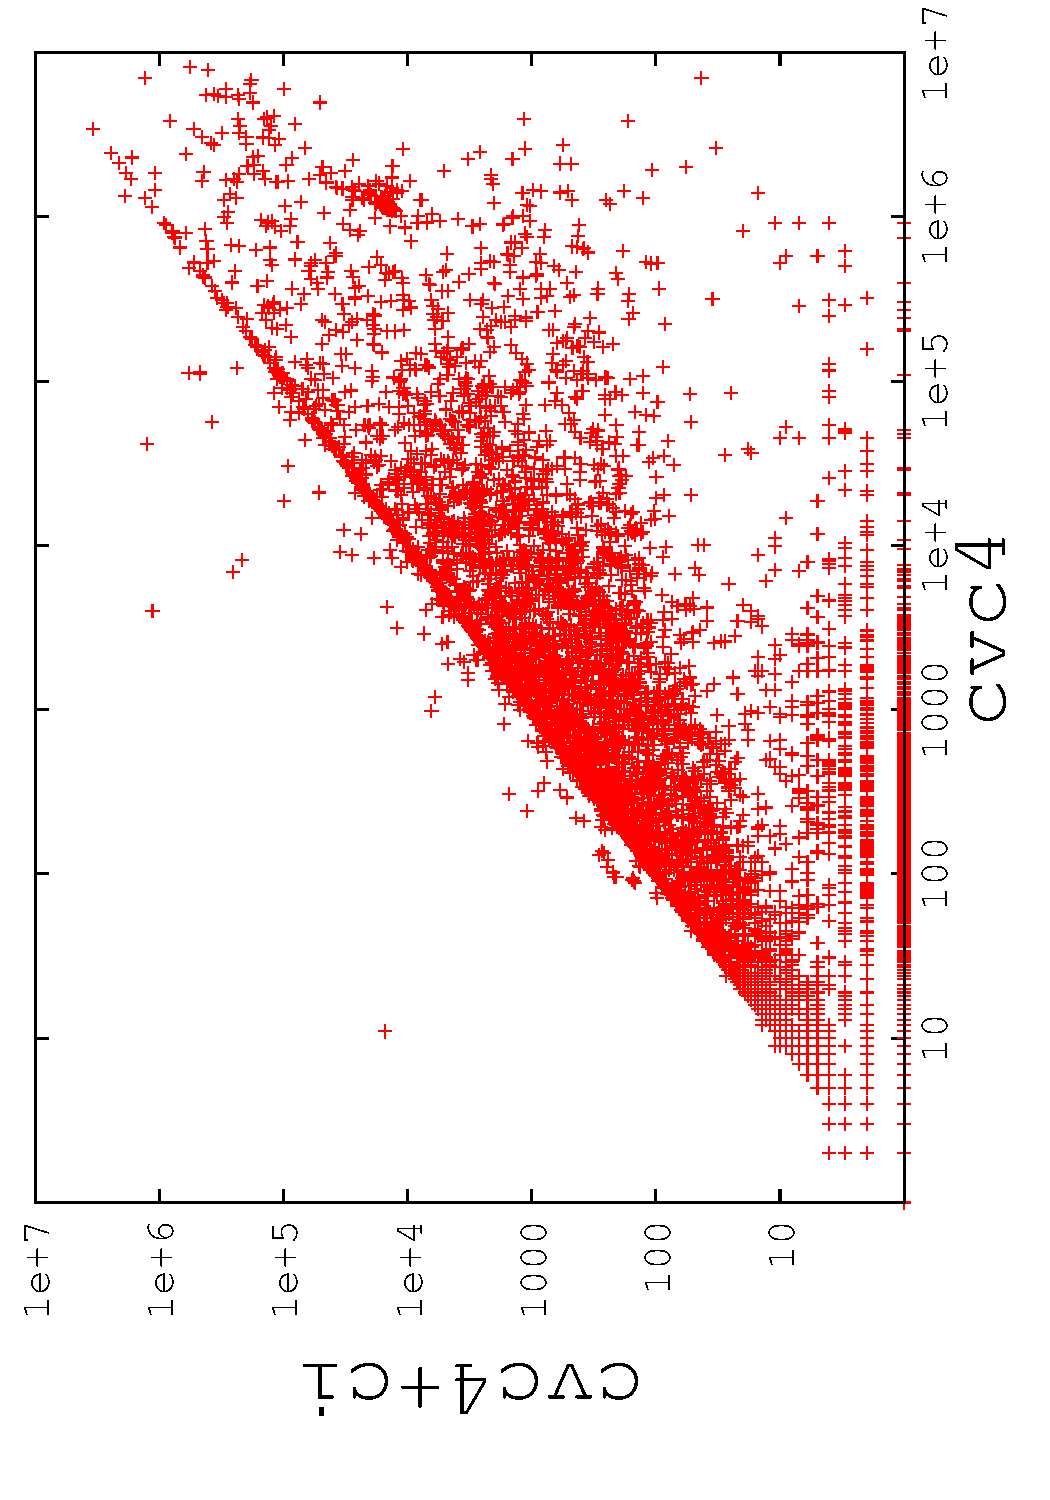
\includegraphics[scale=.22, angle=270]{scatter-cbqi.pdf} 
}
\caption{ Number of instantiations reported by
{\bf cvc4+ci} vs {\bf cvc4} over all unsatisfiable benchmarks.
Data shown on a log-log scale.
}
\label{fig:cbqi-scatter}
\end{figure}

Figure~\ref{fig:results-inst-detail}
gives a detailed summary of the impact of conflict-based instantiation in the SMT solver \cvc
on the SMT-LIB, TPTP, and Isabelle benchmark libraries (further details are given in~\cite{ReynoldsTinelliMoura14}).
Firstly, column 3 shows that \cvc with conflict-based instantiation, as indicated by {\bf cvc4+ci},
solves significantly more benchmarks with respect to \cvc without.
In addition, it uses significantly fewer instantiations overall to solve these benchmarks.
Column 4 gives the aggregate number of instantiation rounds (IR) taken by these configurations
(in terms of Figure~\ref{fig:smtq}, the number of instantiation rounds is equal to the number of calls to $\funcqi$).
Column 5 gives the number of instantiation lemmas returned in these rounds.
We can see that the overall number of instantiations added by {\bf cvc4+ci} is approximately
a factor of five times fewer than {\bf cvc4}.
Overall, {\bf cvc4+ci} solves XXX more benchmarks than {\bf cvc4}
while adding a total of XXX fewer instantiations for doing so.

Columns 6-11 give the percentage of instantiation rounds (IR) taken by the solver 
for which it returns instantiations based on E-matching, a conflicting instance,
or propagating instance(s).
It is interesting to note that conflicting instances are found by \cvc on
XXX\% of instantiation rounds, a percentage that is relatively consistent across all three benchmark sets.
When conflicting instances are not found, propagating instances are found on an additional XXX\% of instantiation rounds.
The number of instantiations added by {\bf cvc4+ci} are by a wide margin those considered during E-matching.

Figure~\ref{fig:cbqi-scatter} gives a scatter plot of the number of instantiations per individual benchmark
across all three sets, where the data is shown on a log scale.
With the exception of a few outliers, {\bf cvc4+ci} consistently considers fewer instantiations,
and in many cases only requires a handful of instantiations to solve benchmarks for which {\bf cvc4}
requires thousands of instantiation lemmas.
It is also interesting to note that several difficult benchmarks can be solved by {\bf cvc4}
without resorting to E-matching at all.
In particular, results from~\cite{ReynoldsTinelliMoura14} showed that XXX benchmarks could be solved {\bf cvc4+ci}
but not by {\bf z3} and {\bf cvc3} where it did not resort to E-matching at all.

\subsection{Challenge: Finding Conflicting Instances}
A key challenge behind conflict-based instantiation
is identifying which instantiations are conflicting in an efficient manner.
A naive approach would be to construct the set of instantiations E-matching, and then check if each one of these instances
was conflicting.
This is highly inefficient, and in fact partially negates our original motivation.
%and in fact partially negates our original motivation for avoiding this construction.
Instead, implementation of conflict-based instantiation in \cvc uses a stronger version of matching
that takes into account the structure of the bodies of quantified formulas.
As a simple example, for the formula $\forall x\, P( x ) \vee R( x )$, we would match
$P( x )$ against ground terms from $E$ that are currently entailed to be equal to $\bot$, but not $\top$.

Another challenge is finding conflicts in the presence of interpreted symbols.
\begin{example}
Let $E$ be the set $\{ f( 1 ) = 5 \}$ and let $\psi$ be $\forall xy\, f( x + y ) > x + 2 \cdot y$.
The instance $f( -3 + 4 ) > -3 + 2 \cdot 4$ is conflicting for $( E, \{ \psi \} )$,
noting that $E, f( -3 + 4 ) > -3 + 2 \cdot 4 \models_{\uflia} \bot$, where $\uflia$ is the combined
theory of uninterpreted functions and linear integer arithmetic.
\qed
\end{example}
In general, finding conflicting instances can be expensive, both because checking entailment modulo theories may be time consuming,
and because matching modulo theories is often not obvious.
For these reasons,
the implementation of conflict-based instantiation in \cvc
considers entailment only modulo equality and uninterpreted functions,
and avoids exponential behavior at the cost of being more incomplete for finding conflicting instances. 

\section{Model-Based Instantiation}
\label{sec:mbqi}

We have seen that E-matching is an incomplete procedure,
that is, when it terminates with no instantiation lemmas, this does not imply that our input is satisfiable.
\emph{Model-based instantiation} is technique that addresses this shortcoming,
which was introduced in the context of modern SMT solving in~\cite{GeDeM-CAV-09},
and has since been implemented in several systems~\cite{Jacobs09,ReyEtAl-CADE-13}.

With model-based quantifier instantiation, the basic idea is
to construct a \emph{candidate model} $\I$ that satisfies $E$, 
and then check whether $\I$ satisfies $Q$ as well.
In other words, $\I$ contains a complete interpretation for all free constants and uninterpreted functions occurring in $E$ and $Q$.
Constructing an interpretation that satisfies the quantifier-free constraints in $E$
is typically possible 
To check whether an interpretation $\I$ satisfies a quantified formula $\forall \vec x\, \varphi[ \vec x ]$ where $\varphi$ is quantifier-free,
it suffices to show that the quantifier-free formula $\neg \varphi^\I[ \vec k ]$ is \emph{unsatisfiable},
where $\varphi^\I$ is the result of replacing each uninterpreted function in $\varphi$
by its interpretation in $\I$.
If $\neg \varphi^\I[ \vec k ]$ is \emph{satisfiable}, we add an instantiation based on the interpretation of $k$ in a model
for this formula.

\begin{example}
Let $E$ be $\{ \neg P( a ), P( b ), \neg R( b ), \neg R( c ) \}$ and let $\psi$ be $\forall x\, P( x ) \vee R( x )$.
We may construct an interpretation $\I$ that satisfies $E$ which interprets:
\[
\begin{array}{rcccccccccc}
P^\I & = & \lambda x. & \ite( & x=a, & \bot, & \ite( & x=b, & \top, & \top  & )) \\
R^\I & = & \lambda x. & \ite( & x=b, & \bot, & \ite( & x=c, & \bot, & \bot  & )) \\
\end{array}
\]
Notice that $P^\I$ was constructed as an if-then-else that has entries corresponding to $P( a ) \Leftrightarrow \bot$
and $P( b ) \Leftrightarrow \top$. Its \emph{default} value (the second occurrence of $\top$ in $P^\I$) was chosen arbitrarily.
Similarly, we fix the existing entries and chose a default value of $\bot$ for $R$.
To check whether $\I$ satisfies $\psi$, we check the satisfiability of:
\[
\neg ( \forall x\, P^\I( x ) \vee R^\I( x ) ) \transform \neg ( P^\I( k ) \vee R^\I( k ) ) \transform \neg ( ite( k=a, \bot, \top) \vee \bot ) \transform ( k = a )
\]
where $k$ is fresh constant.
In other words, after simplification, we find that $\psi$ is not satisfied by $\I$ for all models of $k$ such that $k = a$.
Model-based quantifier instantiation would subsequently return the instantiation lemma $\psi \Rightarrow P( a ) \vee R( a )$.
\qed
\end{example}
Intuitively,
model-based quantifier instantiation adds lemmas that refine candidate models
until they are also a model of $Q$, or otherwise the SMT solver finds a conflict.


\subsection{Impact}
Model-based instantiation often enables SMT solvers to
establish the satisfiability of inputs where exhaustive instantiation is infeasible.
In~\cite{ReyEtAl-CADE-13}, an implementation of model-based quantifier instantiation is used
in conjunction with finite model finding techniques in \cvc.
Figure~\ref{fig:inst-mbqi} shows the impact of these techniques for the 1202
benchmarks from the TPTP library that \cvc finds to be satisfiable.
In both plots, the solid line plots the total number of possible instances of all quantified formulas
in the (smallest) finite model found by \cvc.
For instance, the quantified formula $\forall xyz\, P( x, y, z )$ has $2^3 = 8$ possible instantiations
in a model that interprets the domain of $x,y,z$ each as a set of size $2$.

\begin{figure}[t]
\centering
\subfigure[Number of instantiations without MBQI.]{%
\label{fig:results-tscatter}
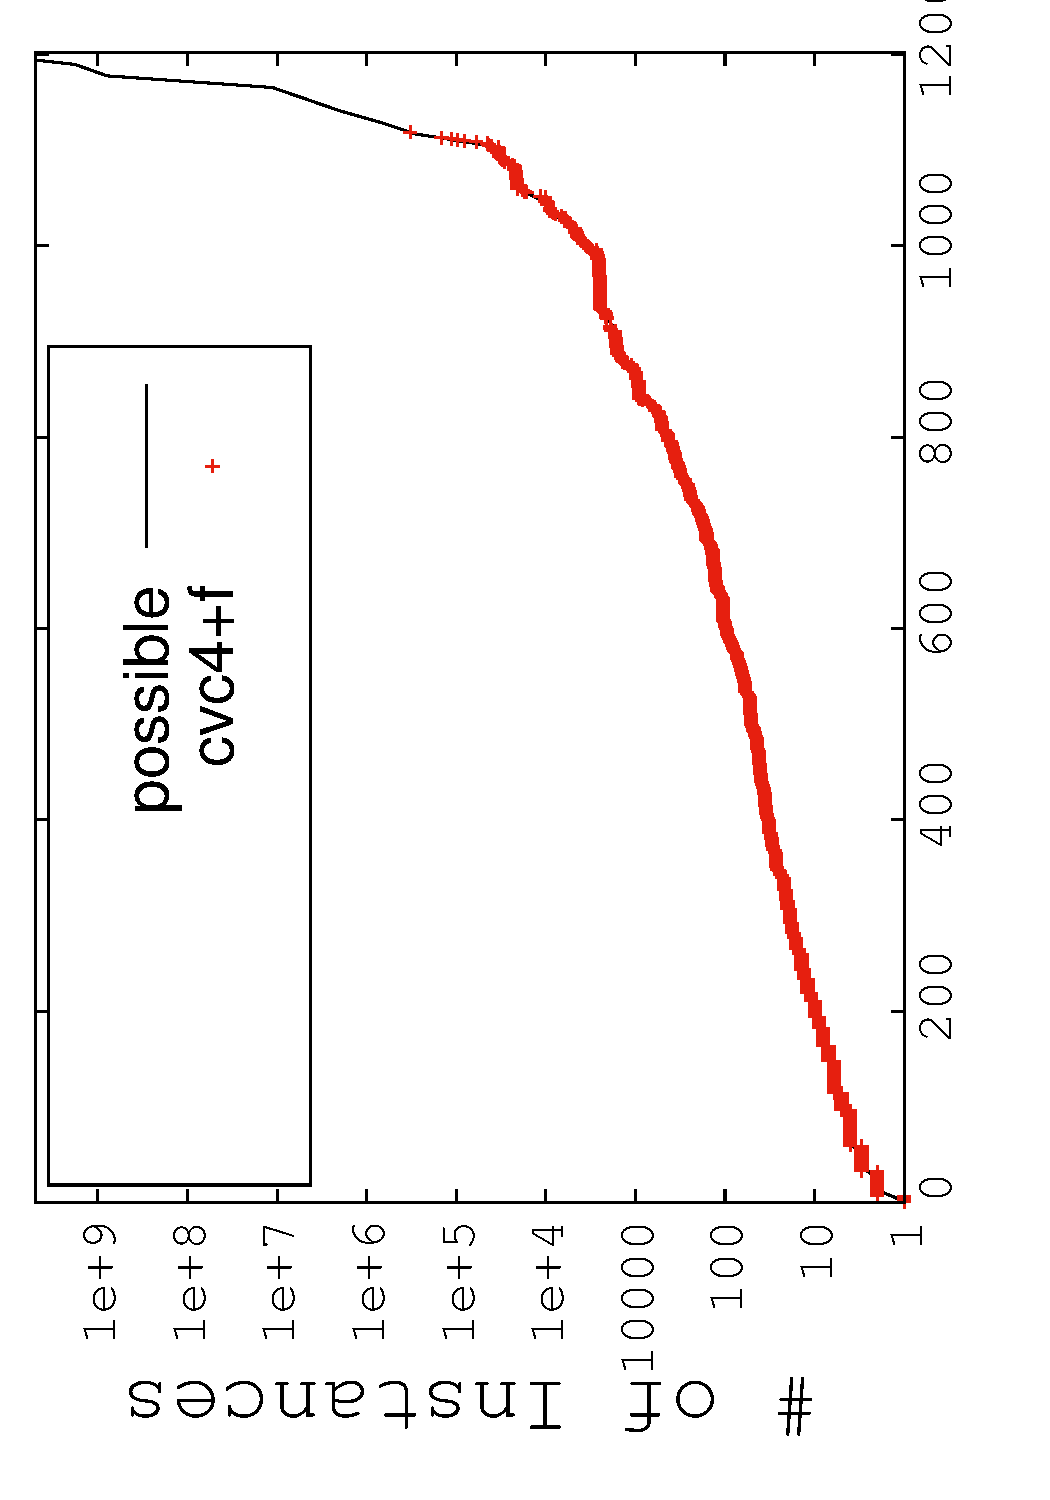
\includegraphics[scale=.22, angle=270]{model-size-nmbqi.pdf} 
}
\quad
\subfigure[Number of instantiations with MBQI.]{%
\label{fig:results-iscatter}
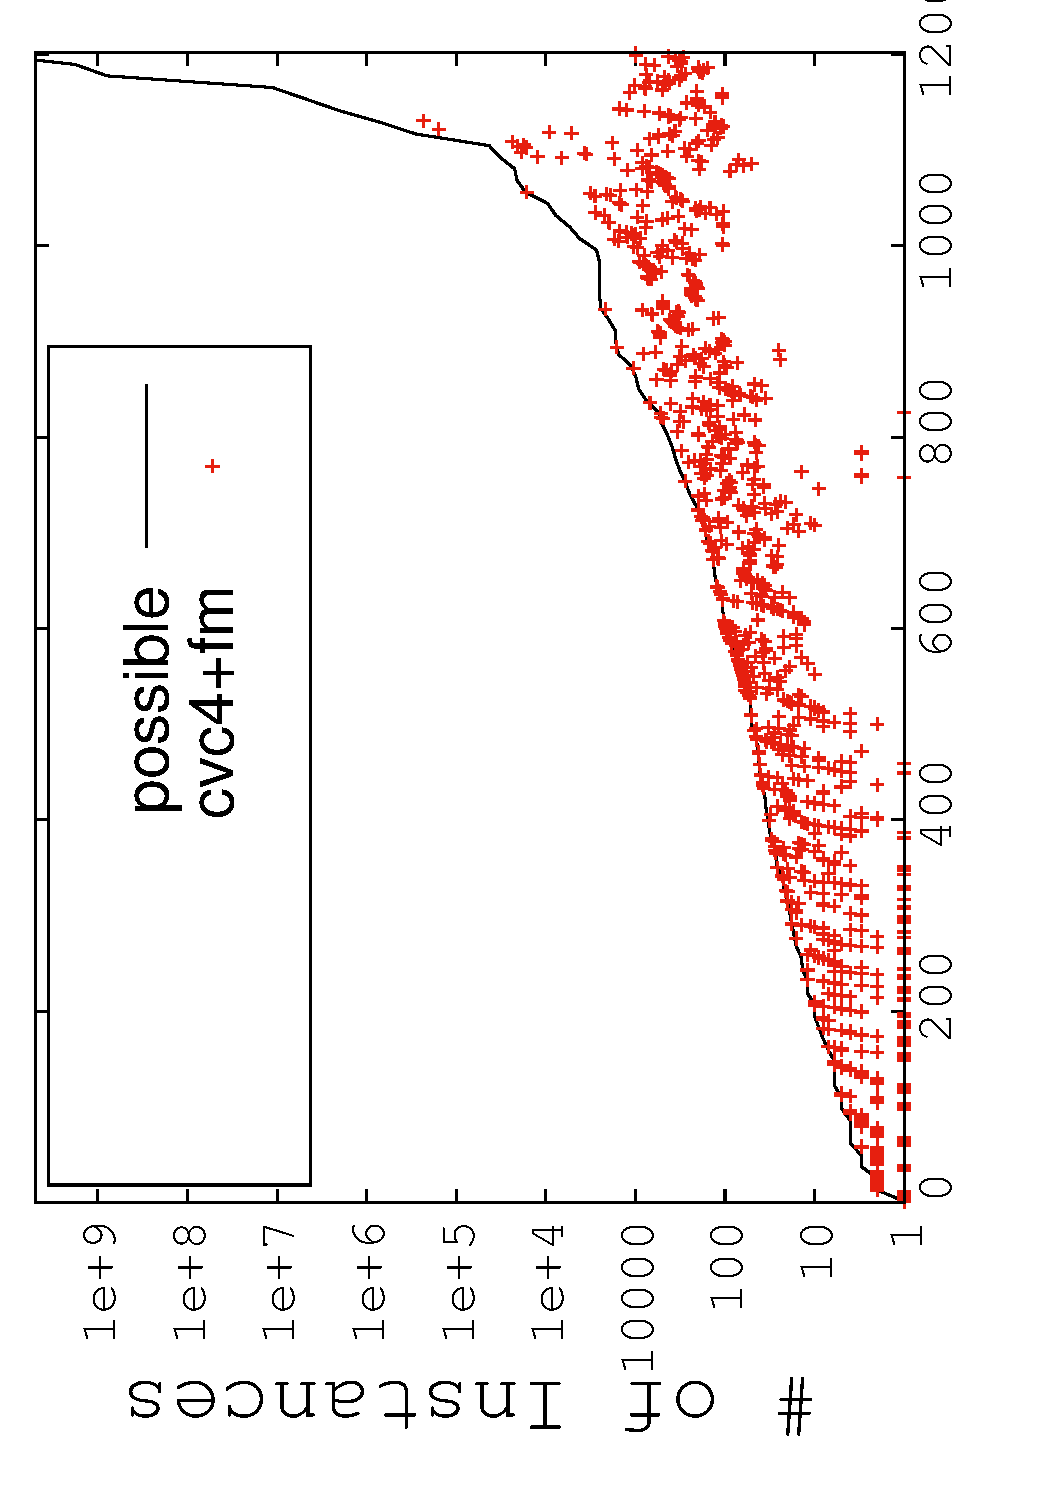
\includegraphics[scale=.22, angle=270]{model-size-mbqi.pdf} 
}%
\caption{
Number of instantiations added by \cvc with and without model-based quantifier instantiation
on satisfiable TPTP benchmarks with a 30 second timeout.
}
\label{fig:inst-mbqi}
\end{figure}

The left plot of Figure~\ref{fig:inst-mbqi} shows the number of instances
added by a strategy {\bf cvc4+f} that exhaustively instantiates all quantified formulas,
where this number coincides with the number of possible instantiations for benchmarks for which
{\bf cvc4+f} terminates with a model.
This plot shows that {\bf cvc4+f} scales up to benchmarks having only around 100k instances;
the maximum number of instances considered by {\bf cvc4+f} on a benchmark it solved was 323k.
In contrast, the right plot of Figure~\ref{fig:inst-mbqi} shows the number of instances
added with model-based quantifier instantiation ({\bf cvc4+fm}).
This strategy solves a superset of the benchmarks solved by {\bf cvc4+f},
solving some benchmarks having more than a billion possible instantiations,
and often adding far fewer than the number of possible instantiations before terminating with a model
as demonstrated by the points in the plot occurring below the solid line.

\subsection{Completeness}
We have now seen that SMT solvers may answer ``unsat" using quantifier instantatiation
when they discover a finite set of instances that are collectively unsatisfiable at the quantifier free,
and SMT solvers may answer ``sat" if they discover a candidate model that satisfies all quantified formulas.
It is worth noting when these solvers are guaranteed eventually to terminate.

Approaches that incorporate model-based instantiation are clearly terminating
when the domains of quantified formulas have a fixed finite interpretation
such in quantified Boolean formulas (QBF)~\cite{janota2012solving},
or quantified bit-vectors~\cite{wintersteiger2013efficiently}.
For quantified formulas over unintepreted sorts,
finite model finding approaches~\cite{ReyEtAl-CADE-13} are generally finite-model complete,
that is guarenteed to terminate with ``sat" when there exists a model that interprets
all uninterpreted sorts as finite sets, and complete for fragments such as Bernays-Schonfinkel
that exhibit a small model property.
More generally, approaches for model-based quantifier instantiation are terminating in cases
where it can be argued that only a finite number of instantiation lemmas will be returned before 
a model is found.
For example, the work of~\cite{GeDeM-CAV-09} examines a class of formulas known as the essentially uninterpreted fragment,
where it can be argued that if a computation of the relevant domain of quantified formulas is finite,
then an instantiation strategy can be made that is complete.
This fragment includes some quantified formulas over infinite domains such as the integers.
%Other fragments that extend Bernays-Schonfinkel have been studied in recent work~\cite{}.

\subsection{Challenge: Constructing Models}
The core challenge to model-based quantifier instantiation is how to construct candidate models $\I$.
As mentioned, common approaches to model-based quantifier instantiation
construct almost constant interpretations for all uninterpreted functions.
This limits their strength both in terms of performance in practice and completeness.

\begin{example}
Let $\psi$ be $\forall xy\, f( x, y ) \geq x \wedge f( x, y ) \geq y$, where $x$ and $y$ are integers.
This formula has a model where for instance $f$ is interpreted as $\lambda xy\, \ite( x \geq y, x, y )$,
but does not have a model where $f$ is almost constant.
\qed
\end{example}

\section{Specialized Instantiation for Theories}
\label{sec:cegqi}

We have seen three classes of general-purpose techniques 
for instantiation for quantified formulas in SMT.
The common thread thus far has been that determining the satisfiability of universally quantified formulas in presence
of uninterpreted functions and theory symbols is challenging, and in fact is undecidable in general.
However, when no uninterpreted function symbols are present and our background theory admits quantifier elimination, 
e.g. linear real and integer arithmetic, then satisfiability 
can be established by a quantifier elimination procedure~\cite{cooper1972,FerranteRackoff79ComputationalComplexityLogicalTheories,Loos93applyinglinear}.
Recent work has adapted quantifier elimination techniques in the context of SMT solving~\cite{monniaux2010quantifier,ReynoldsDKBT15Cav,DBLP:conf/lpar/BjornerJ15},
and has been implemented in SMT solvers
as well as tools that use SMT solvers as a backend~\cite{komuravelli2014smt,DBLP:conf/lpar/FedyukovichGS15}.

Let $\exists \vec x\, \varphi[ \vec x, \vec k ]$ be a quantified formula in a background theory $T$.
Assuming $T$ admits quantifier elimination, we know that this formula is equivalent to some finite disjunction
$\varphi[ \vec t_1, \vec k ] \vee \ldots \vee \varphi[ \vec t_n, \vec k ]$ where $\vec{t_1}, \ldots, \vec{t_n}$ are tuples of terms, possibly containing free constants from $\vec k$.
We may alternatively consider a lazy quantifier \emph{instantiation} procedure for establishing the satisfiability 
$\forall \vec x\, \neg \varphi[ \vec x, \vec k ]$ that considers instantiations of the form 
$\neg \varphi[ \vec t_i, \vec k ]$ where $\vec t_i$ is one of $t_1, \ldots, t_n$.
Assuming only instantiations of this form are considered by the procedure, it is terminating.
Moreover, we may terminate as soon as we discover a set of instantiations $\{ \neg \varphi[ \vec t_{i1}, \vec k ], \ldots, \neg \varphi[ \vec t_{im}, \vec k ] \}$ that either
$T$-unsatisfiable, or are $T$-satisfiable and entail $\forall \vec x\, \neg \varphi[ \vec x, \vec k ]$.
An approach for doing so is given in~\cite{}, which selects instantiations based on the current set of constraints.
\begin{example}

\end{example}

[Results]

\section{Conclusion}
\label{sec:conclusion}

To summarize,
we have seen strategies for quantifier instantiation
based on heuristics, conflicts, and models.
These are summarized in Figure~\ref{fig:smtqi},
a strategy for quantifier instantiation may give priority to instantiations
in the order the techniques are listed, that is, it prefers
returning conflicting instances with highest priority.

\begin{figure}[t]
\begin{framed}
$\funcqi( E, Q )$: \\
\begin{enumerate}
\item[\ ] Do one of the following:
\begin{itemize}
\item If $E \models_T \neg \varphi[ \vec t ]$ for some $\vec t$, $\forall \vec x\, \varphi[ \vec x ] \in Q$, \hfill ({\bf Conflicts})
\begin{enumerate}
\item[\ ] return $( \text{``unknown"}, \{ \forall \vec x\, \varphi[ \vec x ]  \Rightarrow \varphi[ \vec t ] \} )$.
\end{enumerate}
\item Return $( \text{``unknown"}, L )$ based on e.g. E-matching. \hfill {\bf(Heuristics)}
\item Let $\I$ be a model of $E$. \hfill {\bf(Models)}
\item[\ ] If $\I \models \neg \varphi[ \vec t ]$ for some $\vec t$, $\forall \vec x\, \varphi[ \vec x ] \in Q$,
\begin{enumerate}
\item[\ ] return $( \text{``unknown"}, \{ \forall \vec x\, \varphi[ \vec x ]  \Rightarrow \varphi[ \vec t ] \}$ ).
\end{enumerate}
\item[\ ] Otherwise, return $( \text{``sat"}, \emptyset )$.
\end{itemize}
\end{enumerate}
\end{framed}
\vspace{-2ex}
\caption{Summary of techniques for quantifier instantiation in SMT, as subprocedure of Figure~\ref{fig:smtq}.
\label{fig:smtqi}}
\end{figure}

\subsection{Future Work}

There is room to improve upon current implementations of quantifier instantiation in SMT solvers,
both in terms of engineering and theory.
There are many design decisions behind all strategies mentioned in this paper, 
many of which are not mentioned here.
For instance, it has yet to be explored how conflict-based instantiation can be implemented eagerly,
and if it can be efficiently applied in the presence of background theories.
There is also potential for incorporating more advanced constructions 
for model-based quantifier instantiation.

Additionally, there are a number of opportunities to extend SMT solvers with efficient dedicated support for
new fragments of first order logic of interest.
For example, we have seen that specialized approaches for quantifier instantiation in the spirit of Section~\ref{sec:cegqi} 
are highly effective for pure linear real and integer arithmetic~\cite{ReynoldsDKBT15Cav,DBLP:conf/lpar/BjornerJ15}.
There is potential for improving support for quantified formulas over fixed-width bitvectors,
where the bit-precise versions of arithmetic operators are part of the signature supported by many SMT solvers.
We expect analogous techniques for selecting instantiations to be helpful in this case.
It has further yet to be determined how counterexample-guided instantiation techniques can be adapted
for other theories such as non-linear arithmetic, unbounded character strings, finite sets, and floating points, 
which several SMT solvers now support.

E-matching techniques
are often highly effective and well-behaved for fragments where theory symbols are scarce.
Conversely, recent techniques for quantifier instantiation are highly effective for quantifiers containing purely theory symbols.
For tackling problems that depend both on reasoning about theories and uninterpreted functions,
it is yet to fully understood to what extent these techniques can be combined,
and how this combination can be implemented in practice.

\bibliographystyle{abbrv}
\bibliography{main}


\end{document}






